% !TeX program = xelatex
\documentclass[10pt]{beamer}

\usetheme{metropolis}

\usepackage{pgfplots}
\usepgfplotslibrary{fillbetween}
\usepackage{pgfopts}
\usepackage{amsmath}
\usepackage{structuralanalysis}
\usepackage{tikz}
\usepackage{tikz-3dplot}
\usepackage{chngcntr}
\usepackage{wasysym}
\usepackage{mathtools}
\usepackage{alphalph}
\usepackage{xcolor}
\usepackage[showdow=false, en-US]{datetime2}
\usepackage{hyperref}

\newcommand{\highlight}[1]{%
	\colorbox{red!50}{$\displaystyle#1$}}

\setcounter{lecture}{23}
\counterwithin{equation}{lecture}
\makeatletter
\def\user@resume{resume}
\def\user@intermezzo{intermezzo}
%
\newcounter{previousequation}
\newcounter{lastsubequation}
\newcounter{savedparentequation}
\setcounter{savedparentequation}{1}
% 
\renewenvironment{subequations}[1][]{%
	\def\user@decides{#1}%
	\setcounter{previousequation}{\value{equation}}%
	\ifx\user@decides\user@resume 
	\setcounter{equation}{\value{savedparentequation}}%
	\else  
	\ifx\user@decides\user@intermezzo
	\refstepcounter{equation}%
	\else
	\setcounter{lastsubequation}{0}%
	\refstepcounter{equation}%
	\fi\fi
	\protected@edef\theHparentequation{%
		\@ifundefined {theHequation}\theequation \theHequation}%
	\protected@edef\theparentequation{\theequation}%
	\setcounter{parentequation}{\value{equation}}%
	\ifx\user@decides\user@resume 
	\setcounter{equation}{\value{lastsubequation}}%
	\else
	\setcounter{equation}{0}%
	\fi
	\def\theequation  {\theparentequation  \alph{equation}}%
	\def\theHequation {\theHparentequation \alph{equation}}%
	\ignorespaces
}{%
%  \arabic{equation};\arabic{savedparentequation};\arabic{lastsubequation}
\ifx\user@decides\user@resume
\setcounter{lastsubequation}{\value{equation}}%
\setcounter{equation}{\value{previousequation}}%
\else
\ifx\user@decides\user@intermezzo
\setcounter{equation}{\value{parentequation}}%
\else
\setcounter{lastsubequation}{\value{equation}}%
\setcounter{savedparentequation}{\value{parentequation}}%
\setcounter{equation}{\value{parentequation}}%
\fi\fi
%  \arabic{equation};\arabic{savedparentequation};\arabic{lastsubequation}
\ignorespacesafterend
}
\makeatother
\title{AE 737 - Mechanics of Damage Tolerance}
\subtitle{Lecture \arabic{lecture}}
\date{Last Updated: \today\ at \DTMcurrenttime}
\author{Dr. Nicholas Smith}
\institute{Wichita State University, Department of Aerospace Engineering}
% \titlegraphic{\hfill\includegraphics[height=1.5cm]{logo/logo}}

\begin{document}
	
	\maketitle
	\begin{frame}{schedule}
		\begin{itemize}
			\item 19 Apr - Damage Tolerance, Homework 8 Due
			\item 21 Apr - Exam 2
			\item 26 Apr - Exam Solutions, Damage Tolerance
			\item 28 Apr - SPTE, AFGROW, Finite Elements
			\item 3 May - Finite Elements
			\item 5 May - Non-Destructive Testing, Composites, Final Project Due May 10
		\end{itemize}
	\end{frame}
	
	\begin{frame}
		\frametitle{outline}
		\setbeamertemplate{section in toc}[sections numbered]
		\tableofcontents[hideallsubsections]
	\end{frame}

	\section{special topics}
	
	\begin{frame}{special topics}
		\begin{itemize}[<+->]
			\item Damage tolerance is a very broad field, here are some potential things we can discuss for the last few weeks of class
			\item Non-destructive testing (NDT) (some people use "Evaluation" instead of testing, NDE)
			\item Finite element techniques and methods for damage and fracture
			\item Repairing damaged structures
			\item Damage in composite materials
			\item AFGROW
			\item Composite certification 
			\item Other questions?
		\end{itemize}
	\end{frame}
	
	\section{review}
	
	\begin{frame}{group 1}
		Find the fatigue life of 2024-T4 aluminum ($\sigma_f^\prime = 131 \text{ ksi}$, $b = -0.102$) under the following load scenario
		\begin{table}
		\begin{tabular}{ccc}
			\hline Stress Term & Min & Max \\ 
			\hline $\sigma_x$ & 0 & 15 \\ 
			$\sigma_y$ & -5 & 10 \\ 
			$\tau_{xy}$ & 5 & 15 \\ 
			\hline 
		\end{tabular} 
	\end{table}
	\end{frame}
	
	\begin{frame}{group 2}
		Show how to find the cycles to failure for 7075-T6 ($\sigma_f^\prime = 213 \text{ ksi}$, $b=-0.143$, $\epsilon_f^\prime = 0.262$ and $c=-0.619$) with $\epsilon_a = 0.40$ and $\sigma_m = 15 \text{ksi}$
	\end{frame}
	
	\begin{frame}{group 3}
		Use the Boeing method to find an equivalent load cycle for the following load spectrum.
		Repeat this calculation using two different "cycle counting" methods.
		Use material properties for 4340 steel ($p=2.7$, $q=0.84$, $M_T = 70.0$).
		\begin{figure}[H]
			\centering
			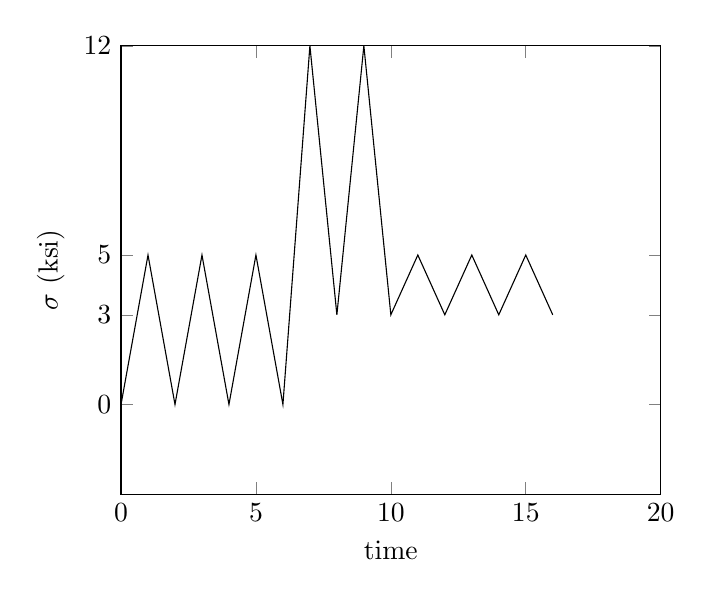
\begin{tikzpicture}
			\begin{axis}[
			domain=0:20,
			samples=200,
			xmin=0,   xmax=20,
			ymin=-3,   ymax=12,
			ylabel=$\sigma$ (ksi),
			xlabel=time,
			ytick={0, 3, 5, 12},
			yticklabels={0, 3, 5, 12}]
			\addplot [color=black,mark=none] coordinates { 
				(0,0)
				(1,5)
				(2,0)
				(3,5)
				(4,0)
				(5,5)
				(6,0)
				(7,12)
				(8,3)
				(9,12)
				(10,3)
				(11,5)
				(12,3)
				(13,5)
				(14,3)
				(15,5)
				(16,3)};
			\end{axis}
			\end{tikzpicture}
		\end{figure}
	\end{frame}
	
	\begin{frame}{group 4}
		For a wide, center-cracked panel with $C=10^{-9}$, $n=4$ and $a_0 = 0.15 \text{ in}$. Assume $\sigma_{YS} = 70 \text{ ksi}$.
		\begin{enumerate}
			\item Integrate to find the crack length after 10,000 cycles of $R=0$, $\sigma_{max} = 10 \text{ ksi}$ loading
			\item Calculate the plane stress plastic zone after an overload of $\sigma = 30 \text{ ksi}$
			\item Find the Wheeler parameter ($\phi$) for the next cycle of $\sigma_{max} = 10 \text{ ksi}$ loading with $m=1.5$
		\end{enumerate}
	\end{frame}
	\section{damage tolerance}
	
	\begin{frame}{definitions}
		\begin{itemize}[<+->]
			\item \textbf{Safe Life}
			\begin{itemize}
				\item Assume cracks are present
				\item Cracks are not inspectable
				\item Use crack growth or fatigue analysis to establish safe life, in which part will not fail
			\end{itemize}
			\item \textbf{Damage tolerant}
			\begin{itemize}
				\item Assume cracks are present
				\item When cracks grow to a sufficient size, they are inpsectable
				\item Inspection cycles are set such that we can be sure crack will not become critical during regular operation
			\end{itemize}
		\end{itemize}
	\end{frame}
	
	\begin{frame}{definitions}
		\begin{itemize}[<+->]
			\item \textbf{Fail safe} multiple load paths, redundancy 
			\item \textbf{Limit load} maximum anticipated load
			\item \textbf{Design load} limit load multiplied by some factor of safety (static design)
			\item \textbf{Operating load} stress spectrum (used for crack propagation/fatigue)
		\end{itemize}
	\end{frame}
	
	\begin{frame}{structural categories}
		\begin{itemize}[<+->]
			\item Single load path - safe life
			\item Single load path - damage tolerant
			\item Multiple load path - externally inspectable
			\item Multiple load path - inspectable prior to failure
		\end{itemize}
	\end{frame}
	
	\begin{frame}{single load path - safe life}
		\begin{itemize}[<+->]
			\item In many structures, multiple load paths are not practical
			\item It is also possible for the critical crack length to be much smaller than is easily detectable
			\item In these cases, safe life design is used to identify a certain number of cycles a part can sustain before it needs to be replaced
			\item This often requires replacing parts pre-maturely
		\end{itemize}
	\end{frame}
	
	\begin{frame}{single load path - damage tolerant}
		\begin{itemize}[<+->]
			\item Redundant load paths are not necessary when a part is easily inspectable
			\item When the detectable crack size is much less than the critical crack length, we can safely inspect a part so that it is only replaced when damage is detected
			\item Many times this damage can be repaired to avoid replacing the part entirely
			\item Ideal for large, expensive parts that are easy to access (inspection and repair)
		\end{itemize}
	\end{frame}
	
	\begin{frame}{multiple load path - externally inspectable}
		\begin{itemize}[<+->]
			\item This is a very common scenario in aircraft (skin/stringer)
			\item In this case, the primary structure is not inspectable
			\item A secondary structure is inspectable
			\item The secondary structure can support a certain number of cycles after failure of the primary structure
			\item Secondary structure can be inspected to observe damage in primary structure
		\end{itemize}
	\end{frame}
	
	\begin{frame}{multiple load path - inspectable prior to failure}
		\begin{itemize}[<+->]
			\item In this case the primary structure is inspectable
			\item Otherwise same as externally inspectable structure
		\end{itemize}
	\end{frame}
	
	\section{inpsection cycle}
	
	\begin{frame}{inspection cycle}
		\begin{itemize}[<+->]
			\item In many industries, an inspection cycle is pre-determined by some governing agency
			\item We have developed all the equations necessary to determine our own
			\begin{enumerate}
				\item Determine loading cycle (or equivalent load cycle using Boeing method)
				\item Determine maximum crack length
				\item Determine initial assumed crack length (minimum detectable crack)
				\item Calculate number of cycles/flights until crack grows to maximum allowable size
			\end{enumerate}
		\end{itemize}
	\end{frame}
	
	\begin{frame}{load cycle}
		\begin{itemize}[<+->]
			\item Be sure to use a consistent cycle-counting method (rainflow or range-pair)
			\item Recall the Boeing method for variable amplitude loads
			\item[] \begin{equation}
			\sum_i \left( z\sigma_{max} \right)_i^{p}N_i = \left( S \right)^{p}
			\end{equation}	
		\end{itemize}
	\end{frame}
	
	\begin{frame}{crack length}
		\begin{itemize}[<+->]
			\item We can use the residual strength curve to set a maximum crack length
			\item We also want to ensure that the crack propagation is still in Region II at this point
			\item Crack growth becomes unstable in Region III
		\end{itemize}
	\end{frame}
	
	\begin{frame}{initial crack length}
		\begin{itemize}[<+->]
			\item What is the smallest crack we can detect?
			\item Liquid penetrant (any material)
			\item Magnetic particle (ferromagnetic materials)
			\item Ultrasonic (any material)
			\item Eddy Current (only for conductive materials)
			\item Radiographic (X-Ray, nearly any material)
		\end{itemize}
	\end{frame}
	
	\begin{frame}{calculate cycles}
		\begin{itemize}[<+->]
			\item We can integrate (analytically or numerically) to find the number of cycles it will take for a crack to grow to critical length
			\item Note that numerical integration is non-conservative, in general
			\item $\Delta N$ should be small enough to give converged solution
		\end{itemize}
	\end{frame}
	
	\begin{frame}{example}
		
	\end{frame}
\end{document}
